% Paper for Learning-Based Controls (ME 537)

\documentclass[letterpaper, 10 pt, conference]{ieeeconf}  % Comment this line out if you need a4paper

\IEEEoverridecommandlockouts                              % This command is only needed if 
                                                          % you want to use the \thanks command

\overrideIEEEmargins                                      % Needed to meet printer requirements.

\usepackage{prg-stuff}

\usepackage{caption}
\usepackage{subcaption}
\usepackage{algorithm}
\usepackage[noend]{algpseudocode}

\makeatletter
\def\BState{\State\hskip-\ALG@thistlm}
\makeatother

%\usepackage{ijcai09}  % style
\usepackage{times}    % font
\usepackage{graphicx} % inserting images
\usepackage{cite}
\usepackage{amsmath}
\usepackage{mathtools} % For math
\usepackage{hyperref}
%\usepackage{enumitem}
\renewcommand{\deg}{\ensuremath{^{\circ}}\xspace}  % why doesn't this work???

\providecommand{\e}[1]{\ensuremath{\times 10^{#1}}}

\graphicspath{ {./figures/} } % Point to the figures directory

%%%%%%%%%%%%%%%%%%%%%%%%%%%%%%%%%%%%%%%%%%%%%%%%%%%%%%%%%%%%%%%%%%%%%%%%%%%

\title{\LARGE \bf 
Active Planning for Defect Detection in the Knife Domain
}

\author{Austin Nicolai, Kory Kraft, Gabriel Hackebeil% <-this % stops a space
%\thanks{*This work was supported by... }% <-this % stops a space
\thanks{\hrulefill}
\thanks{Austin Nicolai and Kory Kraft}
\thanks{Robotics Program, School of Mechanical, Industrial, and Manufacturing}
\thanks{Engineering, Oregon State University, Corvallis, OR 97331, email: }
\thanks{{\tt\small \{nicolaia, kraftko\}@onid.oregonstate.edu}}
\thanks{\hfill}
\thanks{Gabriel Hackebeil}
\thanks{Computer Science Department, School of Electrical Engineering and}
\thanks{Computer Science, Oregon State University, Corvallis, OR 97331, email: }
\thanks{{\tt\small hackebeg@onid.oregonstate.edu}}
}

\begin{document}

\maketitle
\thispagestyle{empty}
\pagestyle{empty}

\begin{abstract}
ABSTRACT TEXT
\end{abstract}


\section{Introduction}

INTRODUCTION TEXT\cite{placeholder}

\section{Related Work}

\subsection{Defect Detection}
Defect detection is necessary within the manufacturing world to ensure both quality and safety. Despite the advanced automated techniques used to manufacture complex products, many products are still manually inspected. The process of manually inspecting parts is tedious and error prone. Furthermore, it can be highly mentally and ergonomically redudant, decreasing employee satisfaction and leading to increased physical strain. Due to resource constraints within companies, it can sap skilled workers away from productive tasks, leading to economic losses. In short, defect detection while important and necessary, is draining.

Attempts and sucesses have been made in automating defect detection, but each defect detection process can be highly dependent upon the good manufactured. We have decided to focus on defects found on small knives. This process currently involves skilled workers taking two hour shifts from their normal job to vizually inspect a small batch of knives for a wide variety of defects. On average, a worker spends 5 seconds inspecting each knife with a 80 percent accuracy rate in detecting defects.

For the focus of this paper, we will focus in on only one type of defect - **defect type**. **Describe defect

\subsection{Computer Vision}

Computer vision, the automated extraction of meaningful information from images, relies on two key components for success: feature extraction and image classification. 

Feature extraction is a necessary to deal with the extremely large datasets that comprise a single image.  For example, a small 64X64 RGB icon has 4096 individual pixels, each of which can be thought of as a unique feature. When looked at as a more complex feature composed of multiple pixels (i.e. the pixels that make up a nose verus an eye), the number of possible features is exponential. 

Feature extraction allows one to cut down the number of features examined from all possible features to a smaller, transformed subset of features that yields the most pertinent information. Feature extraction is different from feature selection in that feature selection simply grabs some subset of the original features and utilizes those.  Feature extraction takes the original features and transforms them into a smaller set of more useful features.

While there are general methods currently in use across machine learning to deal with feature extraction (e.g. PCA) and selection, there are specific methods used in computer vision that take advantage of the image data structure.

Image classification is done using common machine learning techniques for classification. Machine learning comes in two forms: supervised and unsupervised. Unsupervised image classification is done by feeding an algorithm a large data set of images or videos and then allowing the machine to pick out the important features and classify these images. While still in its infancy, deep learning with neural networks have been used successfully. The problem with these algorithms at this stage, is they take a long time to run, and are not yet ready for a real-time vision system. 

Unsupervised learning with image classification requires an expert to label a set of images beforehand. The labeled images are then used to instruct or train the classifier. While more tedious, given a large enough training set, these algorithms can be very efficient and effective.

For example, a real-time vision system for surface defect detection in steel manufacturing was successfully implemented by Jia, et al using standard supervised learning algorithms and a clever feature extraction scheme \cite{steelDefect}. The authors used a rough filter to detect possible edges in the steel and then features are extracted from that according to their length (in pixels), the gray scale constract of seam to adjacent area, the intensity differences between the two sides of the seams, and the mean and varaiance of the seam regions. Using these features, the images were then classified using two standard classification algorithms: K-Nearest Neighbors (KNN) and a Support Vector Machine (SVM). The authors were able to classify the images with greater than 90 perecent accuracy at a rate of 172 images per second, fast enough to detect defects in real-time for a steel rolling machine that could reach speeds of 225 MPH.

A wavelet filter, Gabor filter, and Gabor wavlet filter were successfully used to clasify corrugation defects on rail tracks\cite{railDefect}. In particular, the authors found the Gabor filter to be most successful. The image was first convolved with the Gabor filter at 4 different orientations. Each of these images were then evaluated with an energy distrubution function yielding the mean and variance.  The mean and variance from each filter orientation were assembled to create a feature vector of size 8 for the original image.

\subsection{Adaptive View Planning}

SUBSECTION TEXT

\section{Methods}

\subsection{Data Generation}

In order to accurately detect surface defects in knives, a classifier must be trained. For this classifier to be robust, it must be trained on a large, and comprehensive, set of data.

In order to generate this data, the knives were first filmed under a variety of lighting conditions from multiple angles. From here, still images were extracted to be used for training. The images selected represent many different angles and several lighting conditions. In the image set, there are both positive and negative examples of the defect.

Next, a sliding window technique was used to generate additional training data from the image set. This process is shown in \textit{Figure \ref{fig:data generation}}. First, a user specifies the location of all defect corners. From this, the sliding window is able to automatically determine if it contains a defect and save the windowed image appropriately.

\begin{figure*}
    \centering
    \begin{subfigure}[b]{.32\textwidth}
        \centering
        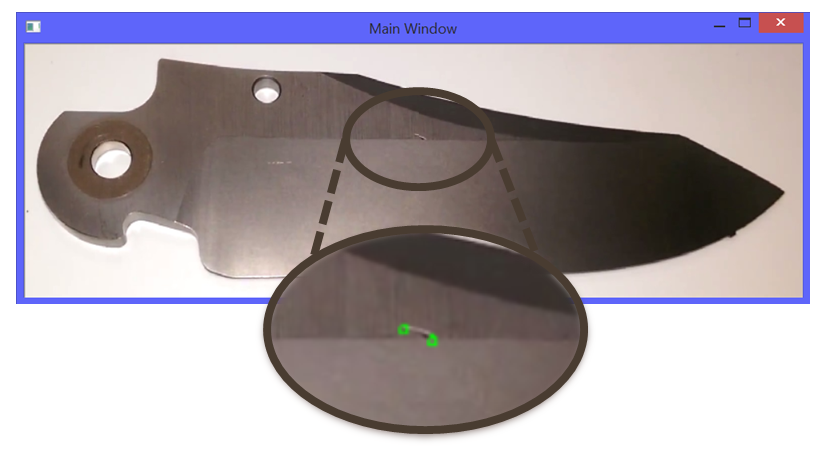
\includegraphics[width=.9\textwidth]{defect_location.png}
        \caption{Selected defect corners}
        \vspace*{2mm}
        \label{fig:defect corners}
    \end{subfigure}
    \hfill
    \begin{subfigure}[b]{.32\textwidth}
        \centering
        \raisebox{8.2mm}
        {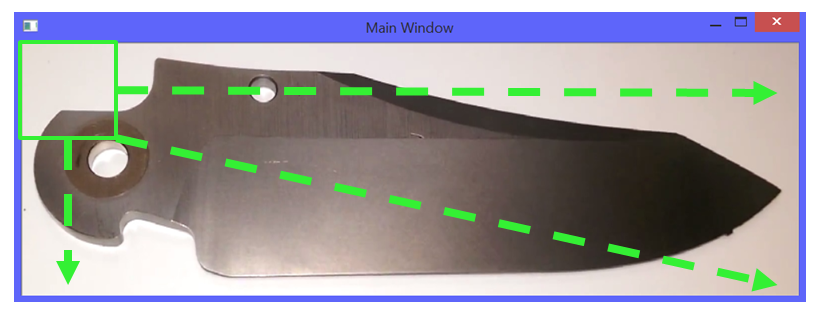
\includegraphics[width=.9\textwidth]{defect_sliding_window.png}}
        \caption{Sliding window}
        \vspace*{2mm}
        \label{fig:sliding window}
    \end{subfigure}
    \hfill
    \begin{subfigure}[b]{.32\textwidth}
        \centering
        \raisebox{1.7mm}
        {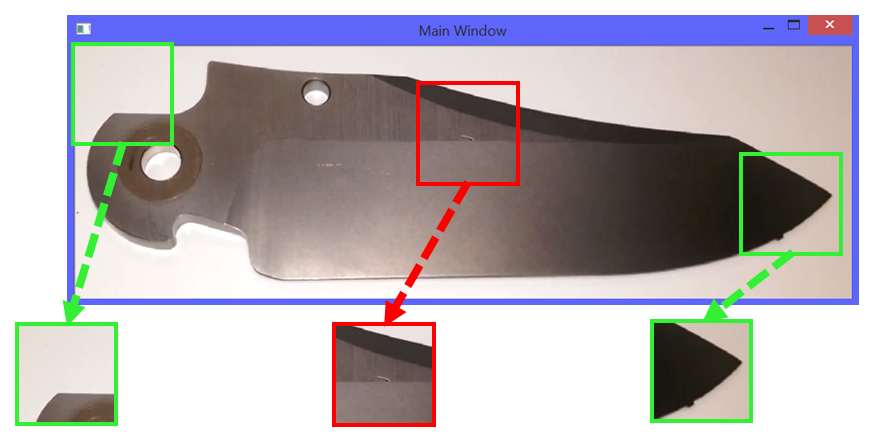
\includegraphics[width=.9\textwidth]{defect_windows.png}}
        \caption{Example labeled windows}
        \vspace*{2mm}
        \label{fig:labeled windows}
    \end{subfigure}
    \caption{Training data generation}
    \label{fig:data generation}
\end{figure*}

\subsection{Computer Vision Algorithm}

The computer vision algorithm employed in this paper was first proposed by ***ADD REFERENCE*** for use in defect detection in railroad tracks. The algorithm uses Gabor wavelet filters to extract features from an input image. The classification is performed by an SVM ***MAKE SURE DEFINED SOMEWHERE*** classifier. A flowchart of the algorithm can be seen in \textit{Figure \ref{fig:vision algorithm diagram}}.

First, the input image is fed through a filter bank. This filter bank consists of Gabor wavelet filters. Four wavelet orientations are used: \textit{0\degree}, \textit{45\degree}, \textit{90\degree}, and \textit{135\degree}. Each orientation is replicated for three different sizes. This yields a total of twelve filters. Next, the magnitude operator is applied to the filtered images. An example of this process can be seen in \textit{Figure \ref{fig:gabor filter bank}}.

The next step is feature extraction for input into the SVM. The features used are the mean and variance of each filtered image. This allows for an image of high resolution to be collapsed down into a manageable feature set. The final resulting feature vector consists of all means and variances. For our algorithm, the feature vector is of length 24.

\begin{figure*}
    \centering
    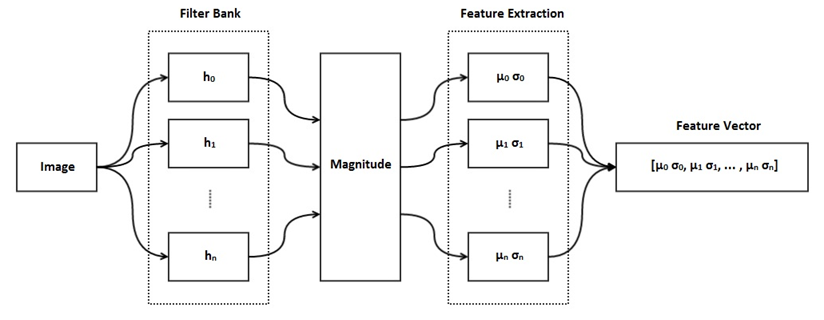
\includegraphics[width=.75\textwidth]{computer_vision_diagram.png}
    \caption{Computer vision algorithm flowchart}
    \vspace*{2mm}
    \label{fig:vision algorithm diagram}
\end{figure*}

\begin{figure}
    \centering
    \begin{subfigure}[b]{.49\textwidth}
        \centering
        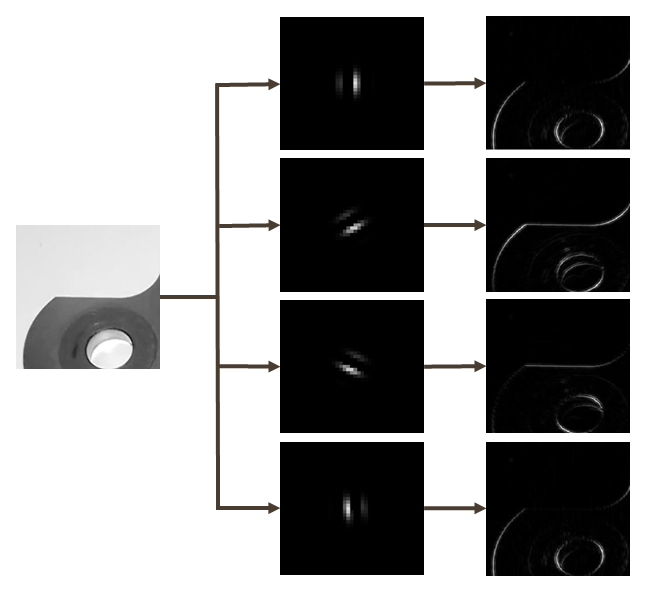
\includegraphics[width=.65\textwidth]{gabor_filter_small.png}
        \caption{Small Gabor filter bank}
        \vspace*{2mm}
        \label{fig:small gabor}
    \end{subfigure}
    \hfill
    \begin{subfigure}[b]{.49\textwidth}
        \centering
        {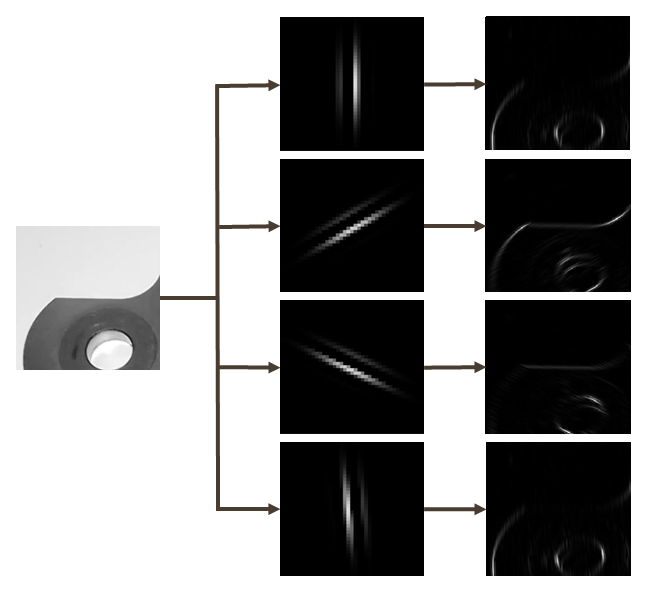
\includegraphics[width=.65\textwidth]{gabor_filter_large.png}}
        \caption{Large Gabor filter bank}
        \vspace*{2mm}
        \label{fig:large gabor}
    \end{subfigure}
    \caption{Gabor filter bank examples}
    \label{fig:gabor filter bank}
\end{figure}

\subsection{View Enumerations}

SUBSECTION TEXT

\subsection{Planning Algorithm}

SUBSECTION TEXT

\section{Results}

RESULTS TEXT

\subsection{SUBSECTION ONE}

SUBSECTION TEXT

\subsection{SUBSECTION TWO}

SUBSECTION TEXT

\section{Discussion}

\subsection{SUBSECTION ONE}

SUBSECTION TEXT

\section{Conclusion}

CONCLUSION TEXT

\bibliographystyle{IEEEtran}
\bibliography{main.bib}


\end{document}

% FIGURE HINTS 
%
%\begin{figure*}
%    \centering
%    \begin{subfigure}[b]{0.3\textwidth}
%        \centering
%        \includegraphics[width=.7\textwidth]{Reflex.jpg}
%        \caption{Reflex agent path}
%        \label{fig:reflex path}
%    \end{subfigure}
%    \hfill
%    \begin{subfigure}[b]{0.3\textwidth}
%        \centering
%        \includegraphics[width=.7\textwidth]{Random.jpg}
%        \caption{Random agent path}
%        \label{fig:random path}
%    \end{subfigure}
%    \hfill
%    \begin{subfigure}[b]{0.3\textwidth}
%        \centering
%        \includegraphics[width=.7\textwidth]{Memory.jpg}
%        \caption{Memory agent path}
%        \label{fig:memory path}
%    \end{subfigure}
%    \caption{Agent paths}
%    \label{fig:agent paths}
%\end{figure*}

% ALGORITHM HINTS
%
%\begin{algorithm}[h]
%\caption{Reflex agent}\label{reflex algorithm}
%\begin{algorithmic}[1]
%\If {$isDirty = true$}
%\State \Return \textit{actionSuck}
%\ElsIf {$facingWall \neq true$}
%\State \Return \textit{actionForward}
%\ElsIf {$facingWall = true$ AND $isHome = true$}
%\State \Return \textit{actionOff}
%\Else
%\State \Return \textit{actionTurnRight}
%\EndIf
%\end{algorithmic}
%\end{algorithm}